\section{An introduction to magnetic confinement fusion}
\label{sec:tokamaks_intro}

Nuclear fusion occurs when light atomic nuclei combine to form heavier elements. This process powers stellar bodies and represents a promising avenue for clean, sustainable energy generation. These reactions, such as the fusion of Deuterium and Tritium nuclei to produce an $\alpha$-particle and a high-energy neutron, release substantial energy with the potential for efficient power generation.

The development of fusion energy has acquired heightened significance in the context of contemporary global challenges. As nations worldwide confront climate change and seek to reduce greenhouse gas emissions, fusion technology offers a carbon-neutral alternative to fossil fuels. Furthermore, fusion power could address the growing energy demands of emerging economies while promoting sustainable development, as it requires minimal fuel resources and produces no long-lived radioactive waste like fission does. The abundance of fusion fuel sources in nature also promises enhanced energy security and reduced geopolitical tensions associated with conventional energy resources. Moreover, nuclear power plants can be scaled to meet the demand of the territory in which they are located, without the need to identify suitable locations to harvest renewable but intrinsically intermitted sources of energy such as solar or wind.

To facilitate fusion reactions, the participating elements must be heated to temperatures sufficient for charged nuclei to overcome their repulsive Coulomb forces. At these elevated temperatures, the matter exists as fully ionized gas, termed \emph{plasma} \cite{chen_introduction_2012}, which must be confined for durations adequate to achieve practical reaction probabilities.

Tokamaks \cite{wesson_tokamaks_2011} are experimental devices that have originated in the 1950s in the USSR; \Cref{fig:tcv_schematic} depicts the TCV machine, which has been the subject of this work. They employ toroidal vacuum chambers for plasma confinement using magnetic field configurations \cite{ariola_magnetic_2008,braams_nuclear_2002,esposito_runaway_2016}. Dedicated coils encircling the chamber generate a \emph{toroidal} magnetic field, while \emph{poloidal} field coils produce an \emph{axisymmetric} poloidal field. This poloidal field serves multiple functions: controlling plasma position and shape while inducing \emph{plasma current}; the plasma must, in fact, carry a current that is instrumental to keep the fusion reaction going, as well as to maintain a reference temperature. Over the decades, tokamaks have contributed to study the behavior of plasma among different types of reactions, as well as to develop the technologies necessary to improve and maintain magnetic confinement. More recent devices, such as the ITER and the JT-60SA machines, incorporate the generation of energy into their project goals.
\begin{figure}[t!]
  \centering
  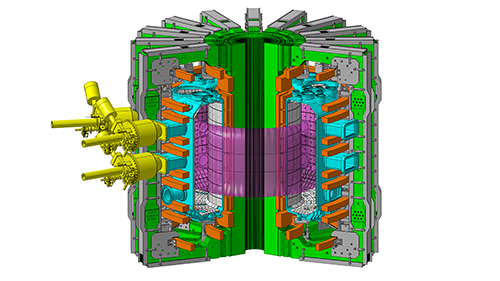
\includegraphics[width=.8\textwidth]{images/ch6/tcv_schematic.jpg}
  \caption{Schematic of the TCV device.}
  \label{fig:tcv_schematic}
\end{figure}

Plasma configurations, characterized by distinct cross-sectional geometries in the poloidal plane, exhibit varying properties regarding stability, performance, and interaction with vessel components. The plasma shape significantly influences the stability characteristics of global \emph{magnetohydrodynamic} (MHD) modes and regulates particle transport phenomena. Furthermore, precise plasma shaping enables optimization of chamber utilization and plasma volume while facilitating controlled management of power deposition from plasma-wall interactions in regions where energy escapes the confined plasma core. To define a plasma shape and its position, two key elements are considered: the \emph{centroid} and the \emph{last closed flux surface} (LCFS).

The centroid is the center of the plasma cross-section along the poloidal plane, and can be either \emph{magnetic} or \emph{geometric}; the type of centroid to consider depends on the specific application at hand. The magnetic centroid is usually involved when it is convenient to approximate the plasma as a filament carrying the plasma current; in that case, the magnetic centroid corresponds to this ideal filament revolving around the vessel. The geometric centroid, on the other hand, can be considered when no such approximation is relevant and the entirety of the plasma cross-section within the vessel must be taken into account. When dealing with magnetic control, which is also the case of this work, the magnetic centroid is usually considered.

Poloidal field coils, running along the torus, generate a poloidal field that induces a \emph{poloidal flux} in the vessel. Along the plasma volume, there are points in which this flux has the same value. Examining the plasma from a poloidal cross-section, one can group this points by flux values, thus identifying \emph{isoflux surfaces}. These run outward starting from the plasma centroid, initially as closed surfaces that enclose one another. The last closed one of these surfaces is identified as the LCFS.

Thus, controlling the plasma shape usually involves tracking reference setpoints for the centroid and the LCFS, expressed as a set of control points \cite{mele_design_2024,tenaglia_unified_2024}. The shape control capabilities directly impact operational parameters and plasma-material interactions, allowing for advanced scenarios that maximize performance while preserving machine integrity. This type of control represents a critical tool for achieving optimal plasma conditions while maintaining operational safety margins. To achieve different plasma configurations in terms of shape, the machine must be equipped with both a vessel large enough to contain them and with a set of coils that can generate the necessary magnetic fields.

The control infrastructure of a tokamak fusion device represents a sophisticated integration of diverse technological components operating across multiple temporal and spatial scales. The hardware architecture encompasses an extensive array of elements: high-power electrical supplies for magnetic field generation, Programmable Logic Controllers (PLCs) for real-time control and safety systems, analog control and diagnostic devices, and server-grade computing systems for data acquisition and processing. This hardware foundation must support both high-bandwidth real-time operations and complex experimental procedures while maintaining strict safety protocols.

The operational complexity extends beyond hardware considerations to include intricate control schemes for plasma magnetic confinement, comprehensive diagnostic systems for plasma state monitoring, and experimental execution frameworks. These systems must operate in concert to maintain plasma stability while facilitating scientific investigation. The human interface component adds another layer of complexity, requiring control rooms staffed by teams of skilled operators managing different aspects of machine operation. The supervision infrastructure must provide interfaces ranging from detailed module-level control to high-level Supervisory Control and Data Acquisition (SCADA) systems, enabling both fine-grained control and system-wide monitoring.

Such operational sophistication demands a robust and well-structured architectural foundation. The control system design must accommodate real-time requirements, ensure fault tolerance, and facilitate system maintenance and upgrades. A distributed systems paradigm offers particularly compelling advantages in this context, providing natural solutions for parallel operation, redundancy, and scalability. This approach enables effective management of the inherent complexity of the system while maintaining the flexibility necessary for experimental physics operations.

\subsection{The Tokamak à Configuration Variable}
\label{sec:tcv}
There are various dimensional parameters that can be used to evaluate the size of a tokamak device; one of these is the \emph{major radius} $R_0$, which is the distance from the center of the torus to the outer wall of the vessel. With a major radius $R_0=\SI{0.88}{\meter}$, TCV is classified as a medium-scale fusion research device. It is operated at the Swiss Plasma Center (SPC) of the École Polytechnique Fédérale de Lausanne (EPFL), Switzerland \cite{lister_control_1997}. The device designation reflects its exceptional plasma shaping capabilities, enabled by an extensive array of independent Poloidal Field (PF) coils in conjunction with a distinctive rectangular vacuum vessel geometry, achieving toroidal magnetic fields up to \SI{1.54}{\tesla}.

The PF coil system, illustrated in \Cref{fig:tcv_layout}, comprises four distinct subsystems.
\begin{itemize}
  \item The \textbf{OH coils}, consisting of a central solenoid (OH1) and an up-down symmetric arrangement of 6 series-connected coils (OH2), provide plasma current drive functionality.
  \item The \textbf{E coils}, comprising 8 independently controlled circuits positioned on the high-field side.
  \item The \textbf{F coils}, featuring 8 independent circuits located on the low-field side.
  \item The \textbf{G coils}, consisting of two up-down symmetric in-vessel coils in anti-series configuration for vertical stabilization of the plasma.
\end{itemize}
The device architecture accommodates removable \emph{baffles} \cite{reimerdes_initial_2021} that enhance plasma core-divertor separation. The configuration depicted in \Cref{fig:tcv_layout} shows the Short-Inner-Long-Outer (SI-LO) baffles arrangement.
\begin{figure}[t!]
  \centering
  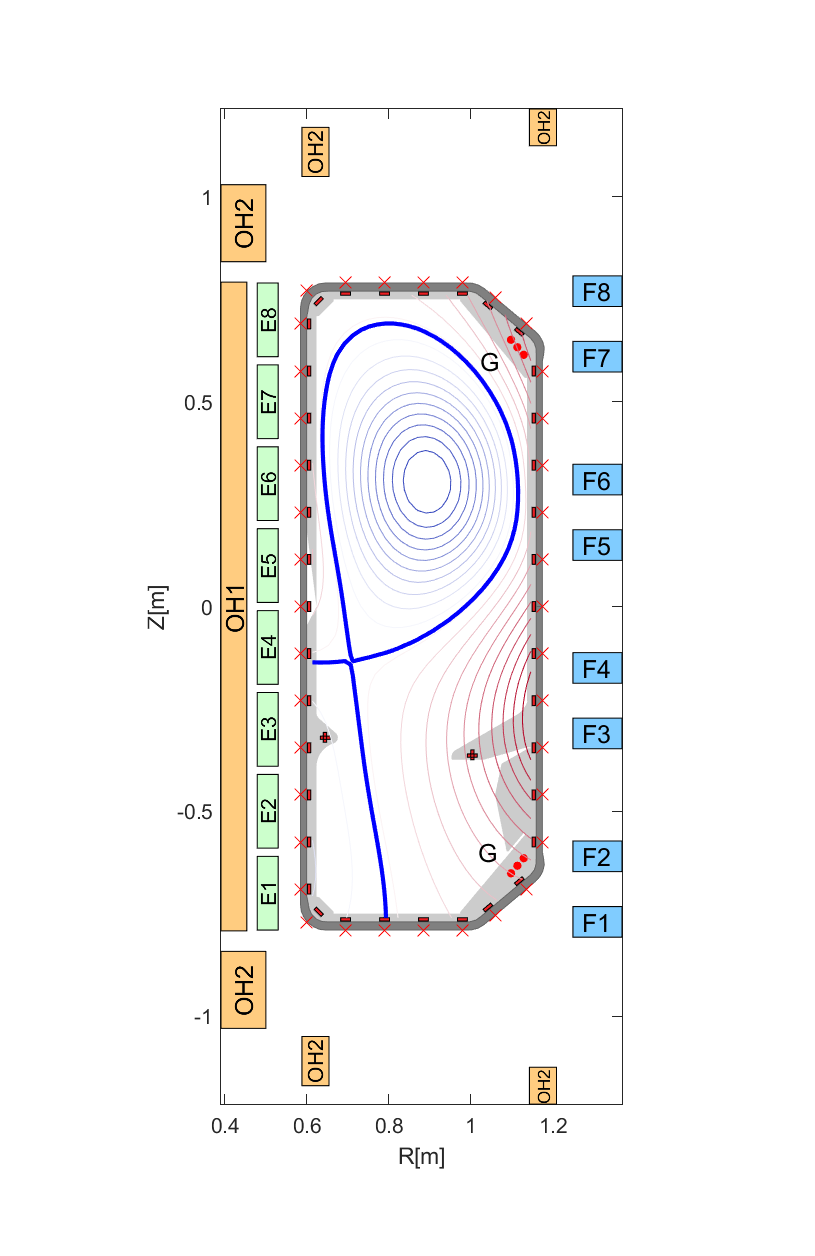
\includegraphics[scale=.6]{images/ch6/tcv_layout.eps}
  \caption{TCV poloidal cross-section with an example plasma configuration (lower single-null). The OH, E, F, and G coils are highlighted in different yellow, green, blue, and red, respectively. Removable baffles appear in the cross-section in gray protruding inward in the bottom part of the vessel.}
  \label{fig:tcv_layout}
\end{figure}

The exceptional plasma shaping capabilities of TCV, combined with its continuously enhanced control architecture, have established this device as a significant contributor to international fusion research \cite{duval_experimental_2024}. Through successive upgrades to both hardware and control systems spanning its three decades of operation, TCV has maintained its position at the forefront of experimental fusion science. Its contributions span multiple international research campaigns \cite{joffrin_overview_2024}, including investigations of advanced plasma configurations and real-time control developments.
